\documentclass[a4paper]{article}
\usepackage[utf8]{inputenc}
\usepackage[spanish, es-tabla, es-noshorthands]{babel}
\usepackage[table,xcdraw]{xcolor}
\usepackage[a4paper, footnotesep = 1cm, width=20cm, top=2.5cm, height=25cm, textwidth=18cm, textheight=25cm]{geometry}
%\geometry{showframe}

\usepackage{tikz}
\usepackage{amsmath}
\usepackage{amsfonts}
\usepackage{amssymb}
\usepackage{float}
\usepackage{graphicx}
\usepackage{caption}
\usepackage{subcaption}
\usepackage{multicol}
\usepackage{multirow}
\setlength{\doublerulesep}{\arrayrulewidth}
\usepackage{booktabs}

\usepackage{hyperref}
\hypersetup{
    colorlinks=true,
    linkcolor=blue,
    filecolor=magenta,      
    urlcolor=blue,
    citecolor=blue,    
}

\newcommand{\quotes}[1]{``#1''}
\usepackage{array}
\newcolumntype{C}[1]{>{\centering\let\newline\\\arraybackslash\hspace{0pt}}m{#1}}
\usepackage[american]{circuitikz}
\usetikzlibrary{calc}
\usepackage{fancyhdr}
\usepackage{units} 

\graphicspath{{../Ejercicio-1/}{../Ejercicio-2/}{../Ejercicio-3/}{../Ejercicio-4/}}

\pagestyle{fancy}
\fancyhf{}
\lhead{22.01 Teoría de Circuitos}
\rhead{Mechoulam, Lambertucci, Rodriguez Turco, Londero, Galdeman}
\rfoot{\centering \thepage}

\begin{document}

\subsection{Datasheet}

\begin{center}
\rule{\textwidth}{1pt}
\textsc{Control de Tonos y Ecualizador TCG3 \textsuperscript{\textregistered}}
\rule{\textwidth}{1pt}
\end{center}

\begin{multicols}{2}

\begin{enumerate}
	\item[1] \textbf{Características}
	\begin{itemize}
		\item Sistema de control de tonos con 3 grados de libertad.
		\item Sistema de amplificación y atenuación sobre la totalidad del espectro audible.
		\item Entrada y salida de audio compatible con conectores de $3.5 \ mm$ mono.
		\item Amplificación y atenuación de hasta $\pm 15 \ db$.
		\item Bajo ruido de entrada.
		\item Cobertura total del espectro audible.
	\end{itemize}
	
	\item[2] \textbf{Descripción}\\
		El \textsc{Control de Tonos y Ecualizador TCG3~\textsuperscript{\textregistered}} es un circuito que permite amplificar y atenuar frecuencias bajas, medias y altas con total independencia entre sí. Posee 3 frecuencias centrales que permiten dicho control. Además cuenta con un regulador de audio, que permite amplificar y atenuar en su totalidad todo el conjunto de frecuencias audibles. El dispositivo requiere una fuente de alimentación para los amplificadores operacionales ($\pm 18 \ V$). Posee entrada y salida audio mono. A su vez cuenta con entradas que permiten de cualquier tipo de señal, ya sea para análisis de esta o calibración del mismo dispositivo.
	
	\item[3] \textbf{Alimentación}
	\begin{table}[H]
		\begin{tabular}{ccccc}
			\hline	
			Tensión & Min & Sugerido & Max & Unidad \\
			\hline
			$V_{in}$\footnote{Valores de tensión dados en amplitud pico-pico.}    & 0 	& 1.5		   & 2	 	& V \\
			$Vcc$       & 10  	& 15       & 18 	& V \\
			$-Vcc$      & -10 	& -15      & -18 	& V	\\
			\hline
		\end{tabular}
	\end{table}
		
	\item[4] \textbf{Valores de interés}
	\begin{table}[H]
		\begin{tabular}{cccc}
			\hline
			\textbf{Banda} & \textbf{Baja} & \textbf{Media} & \textbf{Alta} \\
			\hline			
			$\mathbf{f_{o}}$ & 81.1 Hz & 1.2 kHz & 8.9 kHz \\
			$\mathbf{|Z_{in}|}$ & 30.38 $k\Omega$ & 10.17 $k\Omega$ & 9.92 $k\Omega$ \\
			$\mathbf{Arg\left(Z_{in}\right)}$ & $-42.55^o$ & $-10.74^o$ & $-1.43^o$ \\
			$\mathbf{|Z_{out}|}$ & 8.93 $k\Omega$ & 604 $\Omega$ & 81 $\Omega$ \\
			$\mathbf{Arg\left(Z_{out}\right)}$ & $-90^o$ & $-90^o$ & $-90^o$ \\
			\textbf{Ganancia} & $\pm 12.7 \ dB$ & $\pm 13.7 \ dB$ & $\pm 15 \ dB$ \\
			\hline
		\end{tabular}
	\end{table}

\end{enumerate}
\end{multicols}

\begin{enumerate}
	\item[5] \textbf{Esquemático}\\
\end{enumerate}

\begin{multicols}{2}
\centering
	\begin{figure}[H]
		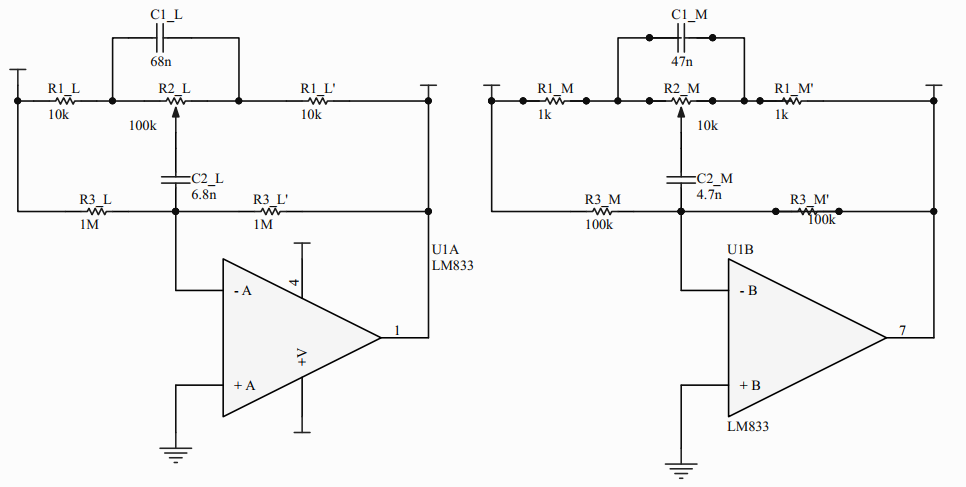
\includegraphics[width=0.5\textwidth]{Imagenes/Schematic-1.png}
	\end{figure}
	\begin{figure}[H]
			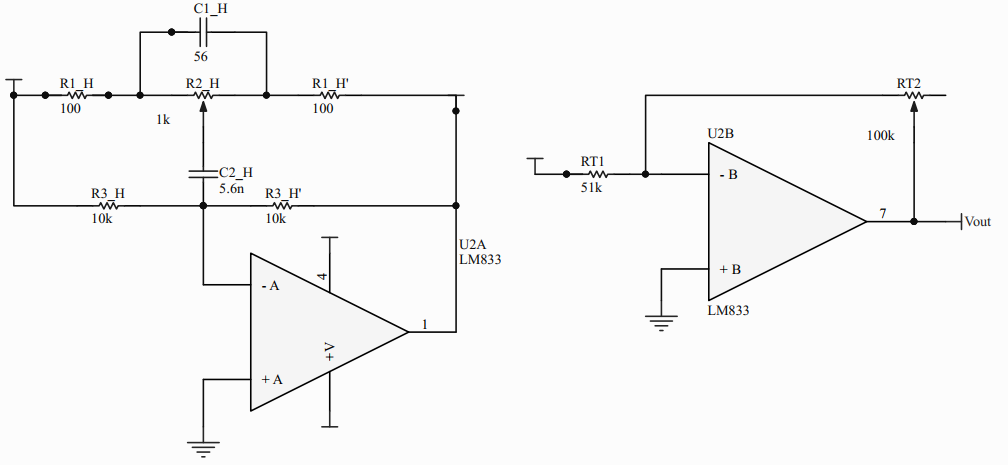
\includegraphics[width=0.5\textwidth]{Imagenes/Schematic-2.png}
	\end{figure}
\end{multicols}

\begin{enumerate}
	\item[6] \textbf{Conexiones de entrada y salida}\\
\end{enumerate}
\begin{multicols}{2}
	\begin{figure}[H]
		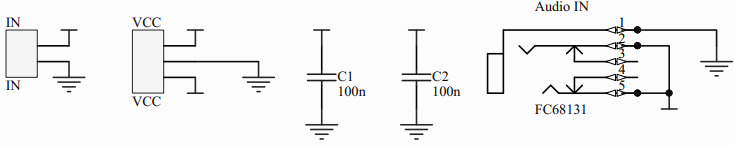
\includegraphics[width=0.5\textwidth]{Imagenes/Input.png}
	\end{figure}
	\begin{figure}[H]
			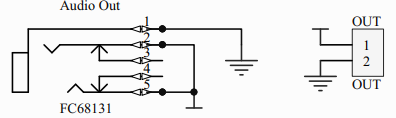
\includegraphics[width=0.3\textwidth]{Imagenes/Output.png}
	\end{figure}
\end{multicols}
 

\end{document}